
\chapter{Results}

In this chapter I will talk more about the implementation details of the \gls{hids}. I will also look into the security of this implementation and what measures can be implemented to improve it. 

\section{System Architecture}
\label{sec:Architecture}

As seen in figure \ref{fig:systemArchitecture} the system itself contains of two components, the scanner and the investigator component. It is split this way to gain flexibility, specifically, that both components can be executed independantly. This has the advantage that the scanner and the investigator don't need to be run on the same system. Also it means that previous results of the investigator can be recreated by running the investigator on the previously captured data. Additionally, if someone is only interested in the results of the scanner, the investigator doesn't need to be run.

Besides the scanner and the investigator which were produced in this thesis, there are four other components which build the environment of the \gls{hids}. There is the \gls{fs} which contains the data in which we are interested. As already mentioned, this could be a mounted device that is directly accessible through the operating system. It could also be run on the disk images of virtual machines or on previously created disk images. To run it on a previously created disk image might be interesting to see a history if an image was taken at multiple different times. Also it could be used on backup images, if backups are made in such a way that they create a disk image. 

Then there is the forensic component. This component is the combination of \gls{tsk} and \gls{pytsk}. The main purpose of this component is the abstraction of the \gls{fs} into python classes which can then be used within the Scanner. This abstraction is important to be compatible to multiple different \glspl{fs}. \gls{tsk} offers a lot of different functionality, in this thesis I am only using the utility that is also used for the fls command described in section \ref{sec:fls}. 

The scanner and investigator are explained in detail in section \ref{sec:flow} and \ref{sec:Investigator}, the database in section \ref{sec:Database} which leaves the alerting component. This component will be part of the section \ref{sec:Investigator}. One component that is not on the diagram is the configuration. This component is special because it influences every other component and at the same time is relatively simple. The configuration is covered in section \ref{sec:Configuration}.

\begin{figure}[ht]
  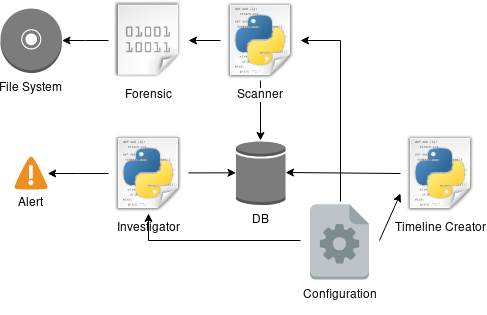
\includegraphics[width=8cm]{../img/Overview_FIDS.png}
  \centering
  \caption{System Architecture}
  \label{fig:systemArchitecture}
\end{figure}

\subsection{Configuration}
\label{sec:Configuration}

The configuration file is provided in \gls{yaml}. \gls{yaml} is a human friendly data serialization language used in many programming languages. Its main advantage over other languages for configuration files is the readability and the ease to extend already existing configuration files. There were more reasons why \gls{yaml} is used documented in section \ref{sec:decisions:config:language}.

\subsubsection{Database Configuration}

The configuration consists of three parts. The first part is the database configuration. Options are to either use the system with a \gls{sqlite} database file, which is the most simple solution, or to use it with a \gls{postgres} database server. For the sqlite configuration only the filename is required as seen in listing \ref{lst:cfg:sqlite}. For a postgres server there needs to be more configuration. The host and port need to be provided, as well as the database, the user and a password as evident in listing \ref{lst:cfg:postgres}. This configuration defines where the data will be sent to and read from in the scanner and investigator parts respectively. As both parts need access to the database this part of the configuration is in a seperate part. It is possible to extend the system to use more \gls{dbms}, it is not part of the scope of this thesis though.

\begin{lstlisting}[language=yaml, numbers=left, caption=SQLite Configuration, label=lst:cfg:sqlite]
sqlite:
	filename: fids_db3.db
\end{lstlisting}


\begin{lstlisting}[language=yaml, numbers=left, caption=Postgres Configuration, label=lst:cfg:postgres]
sqlite:
	filename: fids_db3.db
\end{lstlisting}

\subsubsection{Scanner Configuration}

The second part of the configuration is the part that defines the scanner. An example config can be seen in \ref{lst:cfg:scanner} It consists of one main key which is named scan. If this config entry is missing, the scanner part of the \gls{hids} will not be executed by default. Then it contains the following subkeys:

\begin{itemize}
	\item		\textbf{image\_path} Path to the \gls{fs} that is used for the scan.
	\item		\textbf{scan\_paths} List of paths to scan. Paths will be scanned recursively. "/" will thus scan all the paths.
	\item		\textbf{ignore\_paths} Paths that should not be scanned. Can be a subdirectory of any path in scan paths. The recursion will stop at this path and not continue downwards. Practical if certain directories are not interesting for intrusion detection.
\end{itemize}

\begin{lstlisting}[language=yaml, numbers=left, caption=Scanner Configuration, label=lst:cfg:scanner]
scan:
	image_path: /dev/nvme0n1p5
	scan_paths: 
		[
			"/",
			"/nonExisting",
		]
	ignore_paths: 
		[
			"/temp/"
		]
\end{lstlisting}

\subsubsection{Investigator Configuration}

The investigator configuration is simmilar to the scanner configuration in the way that it contains a top level node called detection. If this is missing the investigator part will not start. As can be seen in listing \ref{lst:cfg:investigator} it has the following subkeys:

\begin{itemize}
	\item \textbf{relevant\_paths} This configuration specifies which paths need to be evaluated for the following changes. 
	\item \textbf{filename\_regex} This configuration specifies the regex which the files need to confirm to.  
	\item \textbf{same\_config} This configuration specifies whether a changed config should result in an alert. Defaults to True.
	\item \textbf{greater} This configuration specifies all the attributes that need to be equal or greater than for the previous run.
	\item \textbf{equal} Simmilar to greater, this configuration specifies all the attributes that need to be equal to the previous run.
\end{itemize}

\begin{lstlisting}[language=yaml, numbers=left, caption=Investigator Configuration, label=lst:cfg:investigator]
detection:
	relevant_paths:[
		"/"
	]
	filename_regex: ''
	greater: [
		"meta_size"
	]
	equal: [
		"meta_creation_time"
	]
	same_config: True
\end{lstlisting}

\subsubsection{Aide Configuration}
\label{sec:aide:config}



\subsection{Database}
\label{sec:Database}

The database is another component that is shared between the scanner and the investigator. As already mentioned, multiple \gls{dbms} can be used in conjunction with this \gls{hids}. In this section I will not focus on the \gls{dbms} used. The database consists of five relations. Firstly, I will explain some reoccuring types, how they are stored and what they represent after that, the relations and then quickly how the different \gls{dbms} can be used. 

Some ideas are not specific to a relation. Most relations contain timestamps and \gls{uuid}. How they are stored can be seen below:

\begin{description}
	\item [Timestamps] To save space, Timestamps are stored as an integer value. This value represents the \gls{unixts}. 
	\item [\gls{uuid}] \gls{id} are stored as \gls{uuid} in their \gls{hex} representation. 
	\item [Enum] \gls{tsk} defines many enums. Most of those enums have an int representation. To save space, this representation is stored in the database. The enums can be viewed in the \gls{tsk} \gls{api} reference. \cite{tsk:file:header}
\end{description}

\subsubsection{FIDS\_RUN}

The run table is relatively simple. It contains a \gls{id} so that each run can be identified. This \gls{id} will be used in the other relations as well to create a link to the run. Besides that it contains a \gls{sha256} hash of the configuration that it was started with. It then contains a start and and end time of this particular run. The table definition is shown in listing \ref{lst:cfg:fids:run}

\begin{lstlisting}[language=sql, numbers=left, caption=Fids Run Table Definition, label=lst:cfg:fids:run]
CREATE TABLE FIDS_RUN(
	id varchar(32), 
	config_hash varchar(64), 
	start_time int, 
	finish_time int, 
	PRIMARY KEY(id)
);
\end{lstlisting}



\subsubsection{FIDS\_ERROR}

With each run there is the possibility of errors. Those errors are stored in this table. It is rather simple as well. Additionally to the run \gls{id} it contains an \gls{id} as well. Next to that it contains a description and a location of where it occured. The table definition is shown in listing \ref{lst:cfg:fids:error}

\begin{lstlisting}[language=sql, numbers=left, caption=Fids Error Table Definition, label=lst:cfg:fids:error]
CREATE TABLE FIDS_ERROR(
	run_id varchar(32), 
	id varchar(32), 
	description text, 
	location varchar(255), 
	PRIMARY KEY(run_id, id)
);
\end{lstlisting}

\subsubsection{FIDS\_FILE}

This table contains most of the information. It again has \gls{id} additional to the \gls{id} of the run. Then it has the path in which the file was located and all the meta information about the file. Most attributes start with meta, while the rest start with name. This is a reference to \gls{tsk} which has multiple structs for meta and name information about each file. I kept the naming of \gls{tsk}, thus more information about each attribute can be found on the \gls{api} reference of \gls{tsk}. \cite{tsk:file:struct} The table definition is shown in listing \ref{lst:cfg:fids:file}

\begin{lstlisting}[language=sql, numbers=left, caption=Fids File Table Definition, label=lst:cfg:fids:file]
CREATE TABLE FIDS_FILE(
	run_id varchar(32),
	id varchar(32),
	path text, 
	meta_addr int,
	meta_access_time int,
	meta_access_time_nano int,
	meta_attr_state int,
	meta_content_len int,
	meta_content_ptr int,
	meta_creation_time int,
	meta_changed_time int,
	meta_creation_time_nano int,
	meta_changed_time_nano int,
	meta_flags int,
	meta_gid int,
	meta_link int,
	meta_mode int,
	meta_modification_time int,
	meta_modification_time_nano int,
	meta_nlink int,
	meta_seq int,
	meta_size int,
	meta_tag int,
	meta_type varchar(255),
	meta_uid int,
	name_flags int,
	name_meta_addr int,
	name_meta_seq int,
	name_name int,
	name_size int,
	name_par_addr int,
	name_par_seq int,
	name_short_name int,
	name_short_name_size int,
	name_tag int,
	name_type varchar(255),
	PRIMARY KEY (run_id, id)
);
\end{lstlisting}

\subsubsection{FIDS\_FILE\_ATTRIBUTE}

In \gls{tsk} each file can contain multiple attributes. Those attributes are stored in this table. It contains the previous \gls{id} and another one for each attribute as each file can have multiple attributes. The attributes contain flags, a name and a type. The flags and the type enums called `TSK\_FS\_ATTR\_FLAG\_ENUM' and `TSK\_FS\_ATTR\_TYPE\_ENUM'. More information available in the \gls{tsk} \gls{api} reference. \cite{tsk:attr:struct,tsk:file:header} The table definition is shown in listing \ref{lst:cfg:fids:file:attr}

\begin{lstlisting}[language=sql, numbers=left, caption=Fids File Attribute Table Definition, label=lst:cfg:fids:file:attr]
CREATE TABLE FIDS_FILE_ATTRIBUTE(
	run_id varchar(32),
	file_id varchar(32),
	id varchar(32),
	flags int,
	tsk_id int,
	name varchar(255),
	name_size int,
	at_type varchar(255), 
	PRIMARY KEY (run_id, file_id, id)
);
\end{lstlisting}

\subsubsection{FIDS\_FILE\_ATTRIBUTE\_RUN}

Attributes can contain multiple data runs. Those data runs are represented in this relation. It contains all the \gls{id} from the attributes and an additional for the run. It then has a block address and a lenght. More information can again be found in the \gls{tsk} \gls{api} reference. \cite{tsk:attr:run:struct} The table definition is shown in listing \ref{lst:cfg:fids:file:attr:run}

\begin{lstlisting}[language=sql, numbers=left, caption=Fids File Attribute Run Table Definition, label=lst:cfg:fids:file:attr:run]
CREATE TABLE FIDS_FILE_ATTRIBUTE_RUN(
	run_id varchar(32),
	file_id varchar(32),
	attribute_id varchar(32), 
	id varchar(32), 
	block_addr int, 
	length int, 
	PRIMARY KEY(run_id, file_id, attribute_id, id) 
);
\end{lstlisting}

\subsection{Shared}

There are other shared components. Mainly the model of the system. It contains of multiple classes for the types. There is one class for each relation. They can parse \gls{tsk} objects and they can parse database rows. This way both the scanner and the investigator can work with the same classes. Except for parsing they don't have any functionality.

